\documentclass{article}

\usepackage{amsmath}
\usepackage{minted}
\usepackage{graphicx}
\usepackage{caption}
\usepackage{subcaption}
\usepackage{mathrsfs}

%Section style
\usepackage{etoolbox} %for configuration of sloppy
\usepackage{xcolor}


\definecolor{secnum}{RGB}{102,102,102}

\makeatletter
    \def\@seccntformat#1{\llap{\color{secnum}\csname the#1\endcsname\hskip 16pt}}
\makeatother
%end section style

\begin{document}

\section{I.2}

\subsection{I.2.1}

We are using the guassian function:
\begin{equation}
    f(x) = a * exp\left(-\frac{(x-b)^2}{2c^2}\right)
\end{equation}
Where:
\begin{align*}
    a &= \frac{1}{\sigma \sqrt{2\pi}}\\
    b &= \mu\\
    c &= \sigma 
\end{align*}
Giving us the full equation:
\begin{equation}
    f(x) = \frac{1}{\sigma \sqrt{2\pi}} * exp\left(-\frac{(x-\mu)^2}{2\sigma^2}\right)
\end{equation}

\subsubsection{Code}
Using matlab we implemented (2) in the following code, giving us the figures \ref{fig:I1.1}

\begin{minted}{matlab}
function [ f ] = gaussjohn( mu, sigma )
    a = 1 / (sigma * sqrt(2 * pi));
    f = @(x) a * exp(-((x - mu)^2) / (2 * sigma^2));
end

fplot(gaussjohn(-1,1), [-10,10])
fplot(gaussjohn( 0,2), [-10,10])
fplot(gaussjohn( 2,3), [-10,10])
\end{minted}

\begin{figure}[h!]
    \centering
    \begin{subfigure}[b]{0.5\textwidth}
        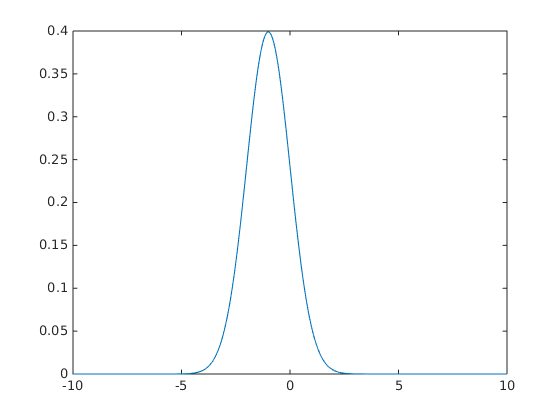
\includegraphics[width=\textwidth]{part1/I211.png}
        \caption{$(\mu, \sigma) = (-1,1)$}
    \end{subfigure}%
    \begin{subfigure}[b]{0.5\textwidth}
        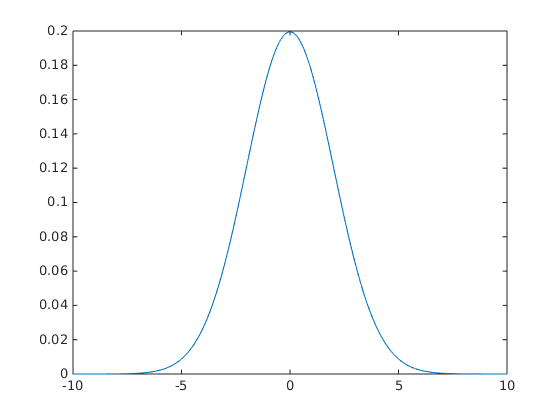
\includegraphics[width=\textwidth]{part1/I212.png}
        \caption{$(\mu, \sigma) = (0,2)$}
    \end{subfigure}
    \begin{subfigure}[b]{0.5\textwidth}
        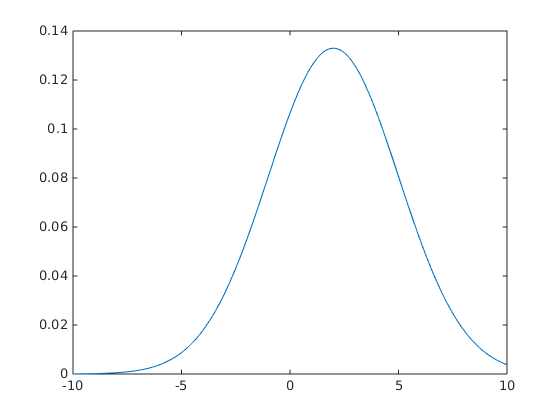
\includegraphics[width=\textwidth]{part1/I213.png}
        \caption{$(\mu, \sigma) = (2,3)$}
    \end{subfigure}
    \caption{Gaussian distribution with varying parameters}
    \label{fig:I1.1}
\end{figure}

\subsection{I2.2}

We created two sets of normal distribution $\mathscr{N}(0,1)$, and extrancted a sample with the distribution of $\mathscr{N}(y \| \mu, \sum)$ 
with mean:

\begin{equation}\label{eq:2.2mean}
    \mu &= (1,2)^T
\end{equation} 
and covariance:

\begin{equation}\label{eq:2.2co}
    \sum &= \left( \begin{array}{cc} 0.3 & 0.2 \\ 0.2 & 0.2 \end{array} \right)
\end{equation}
using the code seen below. This gave us the plots seen on Figure \ref{fig:I2.2}
\begin{figure}[h!]
    \centering
    \begin{subfigure}[b]{0.5\textwidth}
        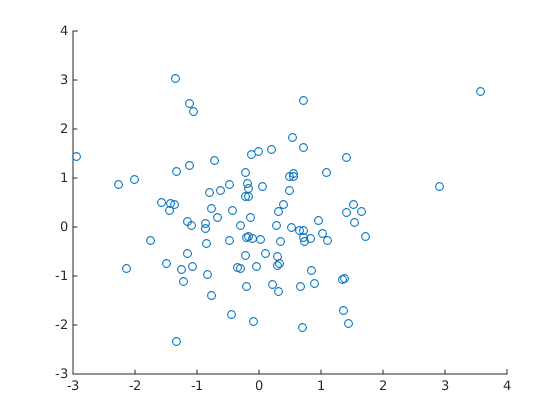
\includegraphics[width=\textwidth]{part1/I221.png}
        \caption{$\mathscr{N}(0,1)$ distribution}
    \end{subfigure}%
    \begin{subfigure}[b]{0.5\textwidth}
        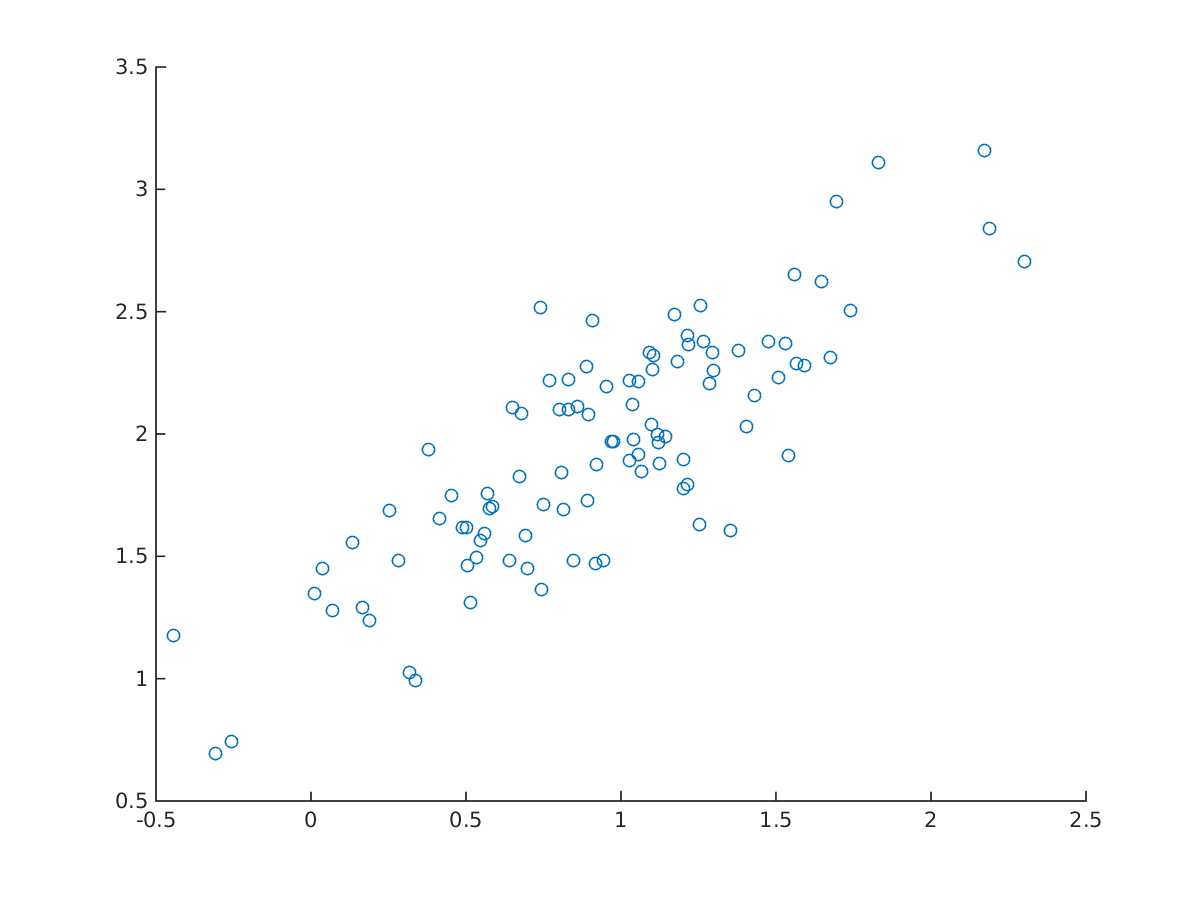
\includegraphics[width=\textwidth]{part1/I222.png}
        \caption{Sample distribution with (\ref{eq:2.2mean}) and (\ref{eq:2.2co})}
    \end{subfigure}
    \caption{Gaussian distribution with varying parameters}
    \label{fig:I2.2}
\end{figure}
\subsubsection{Code}

\inputminted{matlab}{part1/i22john.m}

\subsection{I2.3}


\begin{figure}[h!]
    \centering
    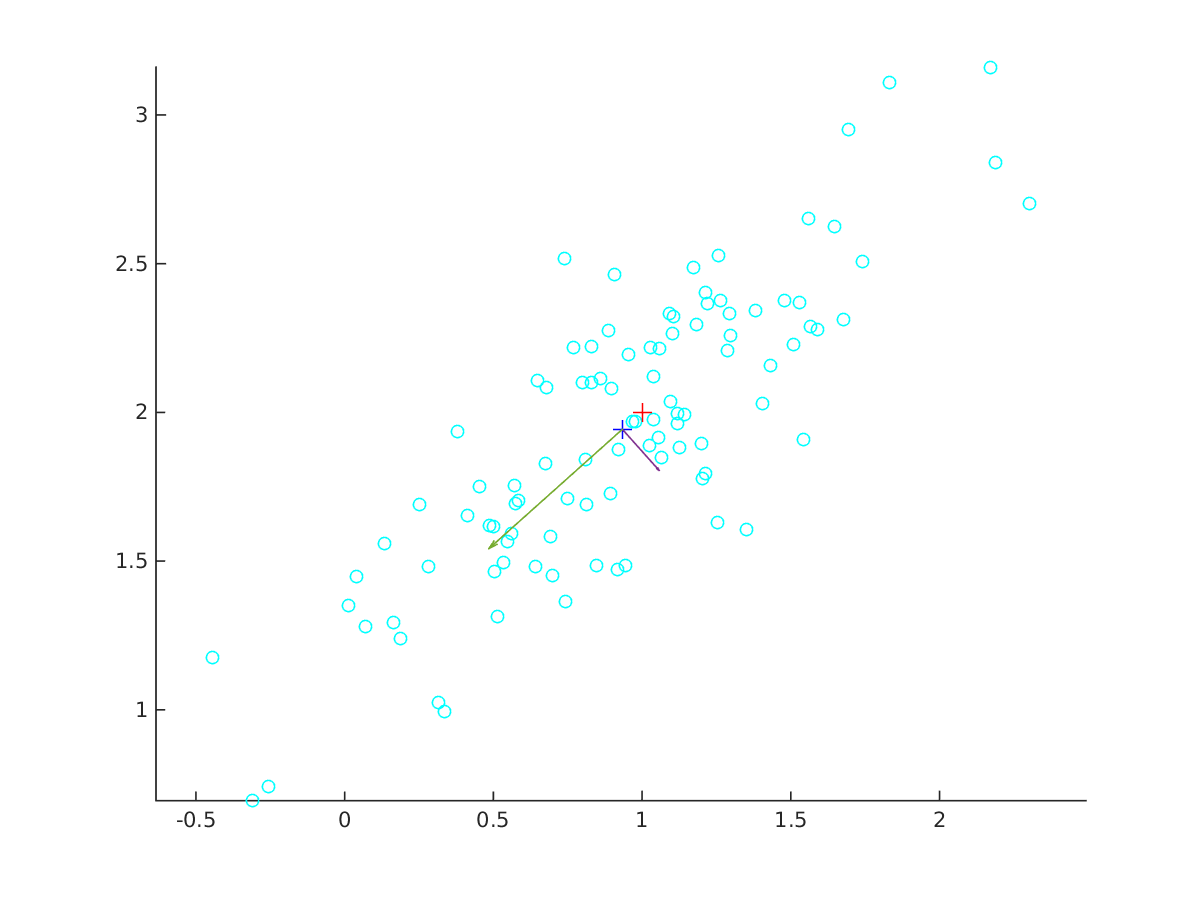
\includegraphics[width=\textwidth]{part1/I231.png}
    \caption{}
    \label{fig:I3.1}
\end{figure}

\subsubsection{Code}

\inputminted{matlab}{part1/i23john.m}

\end{document}
